Das Klimasystem ist ein komplexes und hoch-dimensionales System. Dieses durch ein Modell berechenbar zu machen, ist dementsprechend schwierig und bedarf einiger Abstraktionen. Laut Definition (vgl. Stachowiak in \cite{stachowiak}) sollen Modelle nicht alle Attribute des abgebildeten Systems übernehmen, sondern vielmehr eine Vereinfachung dessen sein. Mit einer kleinst-möglichen und aber notwendig großen Komplexität. Auf Klimamodelle bezogen bedeutet dies, dass man nicht alle einzelnen Bausteine des Klimas durch das Modell abbilden soll, sondern, dass manche Komponenten durch Parameter und Annäherungen abgebildet werden müssen. Ein globales Klimamodell (GCM) liefert im generellen recht gute Aussagen über die Entwicklung des globalen Klimas. Jedoch beruhen diese Ozean-Atmosphären gekoppelten Zirkulationsmodelle, auf einer Parametrisierung der Konvektion, da diese im relativ groben Raster eines GCM nicht simuliert werden kann. Dadurch können grobe Fehler entstehen. (vgl. Stevens \& Bony in \cite{stevensbony}). Es ist aufgrund der Rechenkosten und Rechenzeit jene Herangehensweise, mit parametrisierter Konvektion, im Simulieren großflächiger globaler Klimamodelle  unumgänglich. Großflächige Prozesse des Klimas, wie z.B. der polare Jet, die nordatlantischen Stürme oder auch die stationären planetaren Wellen, werden in den Modellen simuliert.\\
Um Aussagen über die Entwicklung des Klimas in bestimmten Regionen tätigen zu können, müssen GCMs bzw. deren Simulationsergebnisse auf eine entsprechend genaue Auflösung downgescaled werden. Da es auch eine gewisse Rückwirkungen des regionalen Klimas auf das globale gibt sind GCMs eine starke Fehlerquelle in regionalen Klimamodellen, da die Rückkopplung meistens nicht im globalen Modell abgebildet ist (vgl. \cite{woollings_2013}).\\
Da auf der regionalen Ebene die Ortographie sowie die flache Konvektion, die zur Tiefen-Konvektion wird, und die lokalen Kältepools große Auswirkungen auf die Wettererscheinungen haben, müssen diese entweder empirisch-statistisch parametrisiert oder dynamisch berechnet werden. Da ein regionales Klimamodell auch nur endlich genau aufgelöst sein kann, müssen gewisse Aspekte parametrisiert werden. Dies kann wiederum zu Fehlern führen (vgl. \cite{maraun_2010,casanueva_2013}).\\
Wie oben erwähnt ist die Auflösung eines regionalen Klimamodells nur endlich genau: z.B. können Turbulenzen und andere atmosphärische Mikroprozesse häufig nicht von der derzeitigen Maschenweite der Simulationsgitter vollends erfasst und müssen, um grobe Fehler zu vermeiden, statistisch und dynamisch kombiniert downgescaled werden (vgl. \cite{marauntowards}).\\
Als letzte große Fehlerquelle für regionale- und auch globale Klimamodelle sollte die interne Variabilität des Klimas angeführt werden: Alle externen Klimaeinflüsse, wie z.B. der Mensch, oder auch vulkanische und astronomische Erscheinungen führen zu einer Klimareaktion, welche von internen Klimafluktuationen überlagert wird. Da diese Klimaeinflüsse nicht modelliert werden können, ist es auch nicht möglich ein Klimamodell zu entwickeln, welches nicht von zufälligen Fluktuationen dominiert wird (siehe \cite{maraun_value}, Seite 3).\\
\begin{figure}[h]
	\centering
	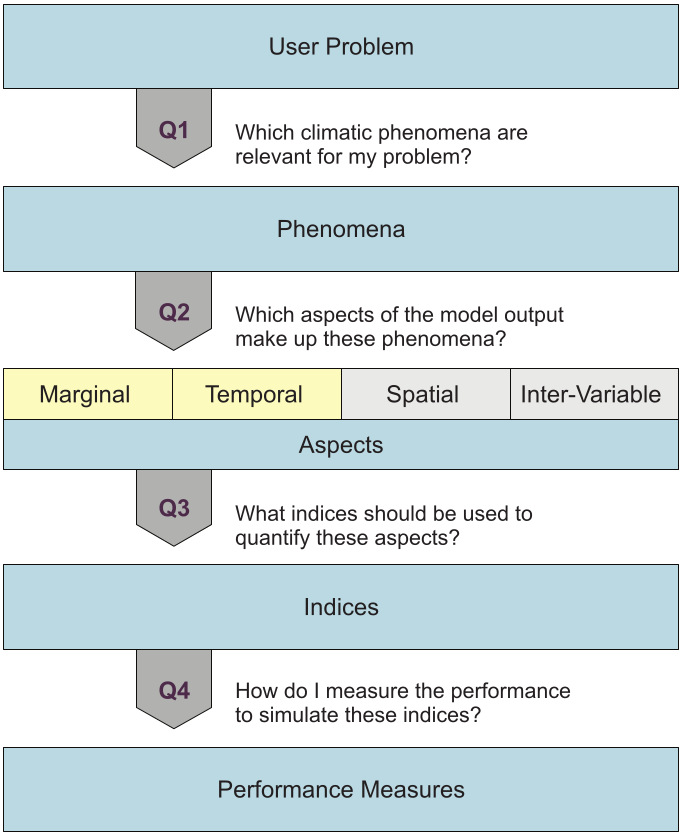
\includegraphics[width=0.5\textwidth]{VALUE.png}
	\caption{Baumstruktur, um eine geeignete Evaluationsmethode zu finden \cite{maraun_value}}
	\label{fig:value}
\end{figure}

Um eine geeignete Evaluierungsmethode zu finden, halte ich mich an die Herangehensweise aus Abb. \ref{fig:value}:
\begin{itemize}
	\item Q1: Starkregenereignisse und Übereinstimmung von Niederschlagsmustern
	\item Q2:
		\subitem{*} Marginal: Intensität
		\subitem{*} Temporal: Jahreszeit bzw. Dauer der Erscheinungen.
		\subitem{*} Spatial: Gewitterzellen sind auf kleinen Arealen zu finden (in den Alpen)
		\subitem{*} Inter-Variable: Temperatur als Begleiterscheinung bei Gewittern.
	\item Q3: Mittelwert der Niederschläge, 99. Quantile, Jahreszeiten, Temperatur-Niederschlagskorrelation, Übereinstimmung der Verteilungskurven und damit dem BIAS der Kurven, räumliche Übereinstimmung mit den Beobachtungsdaten.
	\item Q4: BIAS und relative Fehler (zu den Beobachtungsdaten)
\end{itemize}

Um nun die beiden regionalen Klimamodelle möglichst allgemein miteinander zu vergleichen, werde ich sie über den Mittelwert des Niederschlags, das 99. Quantil über alle zehn Jahre und das 99. Quantil in den vier Jahreszeiten vergleichen. In allen Fällen soll besonders auf die örtliche Verteilung Wert gelegt werden, da diese ein ausschlaggebender Punkt für die Vorhersagekraft regionaler Klimamodelle ist.



